\chapter{Design}

    \section{Introduction}
    This chapter provides an overview of the aspects of BLE that will effect
    the design of any protocols for the technology. Design decisions
    regarding certain aspects of the AODV routing protocol are discussed, and the
    designs for two attendance tracking protocols are outlined, \textit{Roll Call} and
    \textit{Route to Zero}, which are built on top of AODV's route discovery mechanism.

    \section{Bluetooth Low Energy}
    Bluetooth standards are governed by the Bluetooth Special Interest Group (SIG)
    \cite{SIG}. This includes the functionality of the technology, its technical
    operations, certification, interoperability, and standard evolution. In 2009
    SIG announced the Bluetooth Core Specification version 4.0 which
    included BLE. BLE was a radical departure from standard Bluetooth making
    both technologies incompatible with one another. The Bluetooth Core Specification 5.0 \cite{ble_spec}
    was released in December 2016 and provides improved range, speed, and message
    capacity over the previous specifications.

      \subsection{The BLE Protocol Stack}
    BLE devices are divided into three parts: controller, host, and application.
    Each of these parts are subdivided further into layers that provide the various
    functionality that is required to operate. The full stack is illustrated in
    figure \ref{fig:ble_stack}.

    \FloatBarrier
    \begin{figure}[ht]
      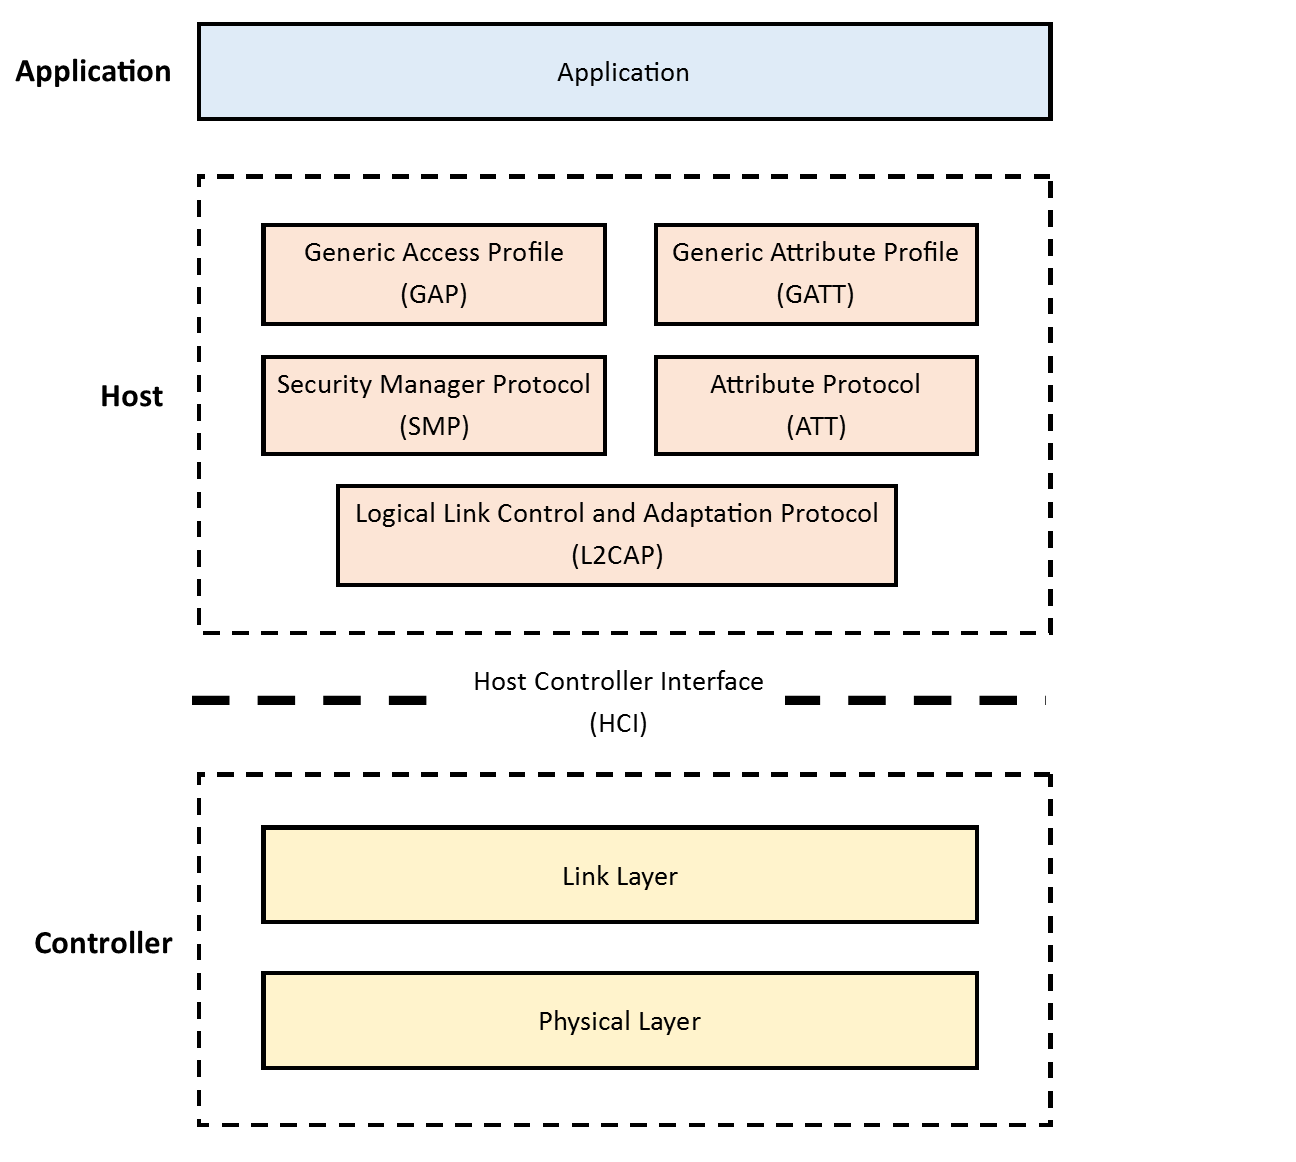
\includegraphics[width=\textwidth]{Images/chapter3/ble_stack.png}
      \caption{The BLE protocol stack}
      \label{fig:ble_stack}
    \end{figure}
    \FloatBarrier

    The application is the highest layer of the stack and is responsible for the
    management of data and implementation of logic that is relevant to the current
    use case.

    The host covers the upper layers of the BLE protocol stack and includes both
    protocols and profiles which are described in more detail below.

    The controller is comprised of the two lowest layers in the stack: the physical
    layer and the link layer.

    The host can communicate with the controller through the Host Controller Interface
    (HCI). The HCI decouples the host and controller, allowing them to be swapped
    without affecting the other. It exposes enough BLE functionality that allows
    the host to perform operations such as scanning and advertising.

      \subsection{Physical Layer}
    The physical layer is comprised of a device's radio, which performs the
    modulation and demodulation of analog signals. The radio uses the
    ISM frequency band with 40 channels, from 2.4 GHz to 2.4835 GHz. Three of these
    channels are used for advertising, and the remaining 37 are used for
    connections. The advertisement channels are located at the start, middle,
    and end of the band. If any single advertisement channel is blocked, the others
    are likely to be free due to the frequency difference in channel placement.
    For this reason, advertising on all channels is recommended for any single
    advertisement packet.

      \subsection{Link Layer}
    The Link layer (LL) directly interfaces with the physical layer and is a combination
    of hardware and software. The LL manages Bluetooth Device addresses, 48 bit
    values which uniquely identify devices. It is also in charge of establishing
    connections. In the case of connections, the LL manages connection intervals
    and is capable of configuring encryption. Consequently, it defines the following
    roles for devices:

    \begin{itemize}
      \item Advertiser - a device which sends advertisement packets
      \item Scanner - a device which scans for advertisement packets
      \item Master - a device which initiates and manages connections
      \item Slave - a device which accepts connection requests
    \end{itemize}

    \subsection{Protocols}
        \subsubsection{Attribute Protocol}
    The Attribute Protocol (ATT) is a transport protocol which defines a
    basic data unit and how it can be exchanged between devices.

    The \textit{attribute} is the basic data unit of the protocol and is composed
    of three elements:
    \begin{itemize}
      \item a 16 bit handle - uniquely identifies an attribute.
      \item a UUID - defines the type of attribute.
      \item a value - a data value of a certain length.
    \end{itemize}

    The protocol is client-server focused. Devices can operate as servers, storing
    attributes in non-volatile memory, and clients can use the protocol to send
    read and write requests to servers. Clients specify the attribute they wish to
    read or write using the attribute's handle value.

        \subsubsection{Security Manager Protocol}
    The Security Manager Protocol (SMP) provides functionality for devices
    to generate and exchange security keys. It defines the following two roles:
    \begin{itemize}
      \item Initiator - the link layer master
      \item Responder - the link layer slave
    \end{itemize}
    The SMP provides support for \textit{Pairing}, \textit{Bonding}, and
    \textit{Encryption Re-establishment}.
    In pairing, devices generate a temporary common security encryption key which is
    used to switch to a secure encrypted link. In bonding, the pairing procedure
    is completed, followed by the generation and exchange of permanent security
    keys. Bonding establishes a permanent bond, as the keys are stored in non-volatile
    memory. Encryption Re-establishment defines how the keys generated during
    the bonding process can be re-used in future connections.

        \subsubsection{Logical Link Control and Adaptation Protocol}
    The Logical Link Control and Adaptation Protocol (L2CAP) is responsible for
    transporting data for higher layer protocols, it is responsible for the
    fragmentation and recombination of packets, and L2CAP performs quality of service
    management for higher layer protocols.

      \subsection{Profiles} \label{profiles}
    Profiles in BLE encapsulate basic modes of operation or specific use cases
    required by devices. Profiles are definitions of how a protocol should be
    used. The Generic Access Profile (GAP) and the Generic Attribute Profile (GATT)
    are the two main profiles in BLE which are fundamental to ensure interoperability
    between devices from different vendors.

        \subsubsection{GAP}
    At its core, GAP allows devices to discover one another, establish connections,
    and broadcast data. GAP defines four roles which are higher level versions
    of those specified by the Link layer, and are as follows:
    \begin{itemize}
      \item Broadcaster - periodically sends out advertising packets with data.
      \item Observer - periodically scans for advertising packets.
      \item Central - initiates connections with peer devices (link layer Master).
      \item Peripheral - establishes connections with centrals (link layer slave).
    \end{itemize}
    A set of modes are also defined by GAP which are a further refinement of roles
    and relate to device discoverability and connectibility.

        \subsubsection{GATT}
    GATT is the top most layer in the BLE stack and deals with data exchanges between
    devices. It is built on top of the ATT and defines a basic data model and functions that allow devices to discover,
    read, write, and push data between one another. The Bluetooth SIG has developed
    a wide range of GATT profiles including:
    \begin{itemize}
      \item Cycling Speed and Cadence Profile - transfer speed and cadence data from
      bicycle sensors to a phone.
      \item Glucose Profile - transfer glucose levels over BLE.
      \item Health Thermometer Profile - transfer body temperature readings over BLE
    \end{itemize}
    GATT is not required for an AODV implementation as all necessary data can
    be transmitted in packets, and host data is irrelevant to other nodes.

      \subsection{Intervals and Windows}
    When a device has the broadcaster role, advertisement packets are sent
    periodically on each of the three advertisement channels. The time interval
    between the sending of advertisement packets is known as the \textit{advertisment
    interval}. This interval is comprised of a fixed interval and a random delay.

    The fixed interval can be set from 20ms to 10.24s, in steps of 0.625ms. The
    random delay is a value from 0ms to 10ms that is automatically added by the
    link layer. The purpose of this random delay is to reduce collisions between
    the advertisements of different devices.

    When a device has the observer role, the device scans each of the three
    channels periodically. The time interval between the scanning of each channel
    is known as the \textit{scan interval} and the time spent scanning each
    channel is called the \textit{scan window}.

    Radio duty cycling is accomplished by reducing the scan interval and scan window.
    In the context of attendance tracking, the window is always set to the minimum
    possible value, while the interval can be set to the maximum possible value. This
    means that the radio duty cycling preamble has to be at least as long
    as the maximum scan interval.

    \FloatBarrier
    \begin{figure}[ht]
      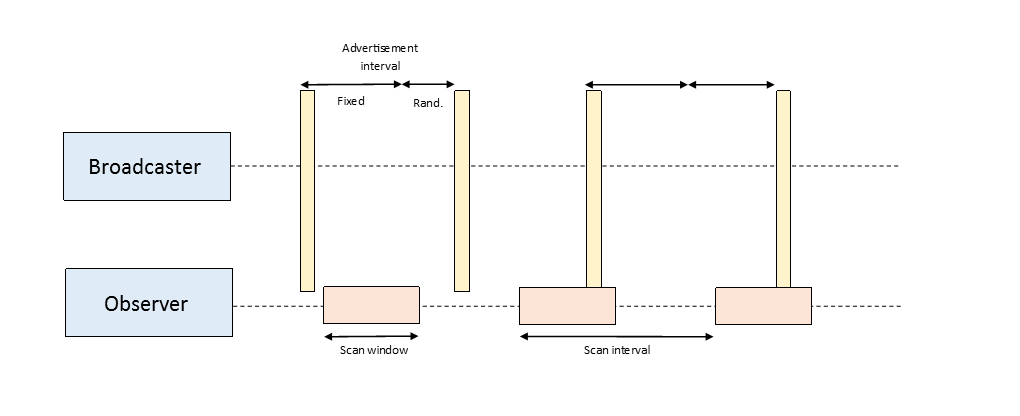
\includegraphics[width=\textwidth]{Images/chapter3/ble_intervals.png}
      \caption{BLE Broadcaster and Observer}
      \label{fig:intervals}
    \end{figure}
    \FloatBarrier

    Figure \ref{fig:intervals} shows two devices with the broadcaster and observer
    roles. It illustrates the importance of interval and window selection, as an
    observer's scan window must overlap with a broadcaster's advertisement
    interval in order to receive the advertisement data. However, the shorter
    the interval and longer the window, the more power is consumed by the radio.

    The designs featured in this section make use of devices with both the
    broadcaster and observer roles. This is to avoid the overhead of establishing
    connections which are unnecessary if a very low number of packet exchanges
    are sufficient, and device location is not guaranteed with each use of the
    application.

      \subsection{Connections}
    Connections are a sequence of data exchanges between central and peripheral
    devices at predefined times. Connections are established by the central
    device scanning neighbouring nodes and identifying if any are currently
    accepting connection requests. If a suitable peripheral is identified, the
    central sends a connection request packet which contains the following:
    \begin{itemize}
      \item Frequency hop count - determines the hopping sequence that will be followed
      by both devices throughout the connection period.
      \item Connection interval - the time between two consecutive connection
      events.
      \item Slave latency - the number of connection events a peripheral can ignore
      without causing a disconnection.
      \item Connection supervision timeout - the maximum time between two received
      data packets before the connection is considered lost.
    \end{itemize}

    Devices can perform a pairing or bonding procedure at the beginning of connections
    using the SMP.

    No connections are established in the attendance tracking protocols outlined in
    this section as the AODV control packets fit within a single advertisement
    packet, and continuous and frequent communications on the level of BLE connections
    is not required, making it an unnecessary overhead.

      \subsection{BLE Data Packets}
    The Packet data unit for the advertising channel (called the Advertising
    Channel PDU) includes a 2-byte header and a variable payload from 6 to 37
    bytes which is illustrated in figure \ref{fig:ble_pkt}. The header includes the actual
    length of the packet and the PDU type. The payload length depends on the
    advertising PDU type. For beacon-like devices, and for attendance tracking,
    the PDU type used is the \textit{ADV\_NONCONN\_IND} type. This type indicates
    a non-connectable advertisement, which means central devices will not attempt
    to establish connections with it.

    The PDU payload includes a 6 byte Bluetooth MAC address, leaving 31 bytes
    for advertisement data structures. These advertisement structures each contain
    a type, length, and data section. The types of these structures are pre-defined
    and the most commonly used include service UUIDs, shortened and complete
    local names, and manufacturer specific data.

    \FloatBarrier
    \begin{figure}[ht]
      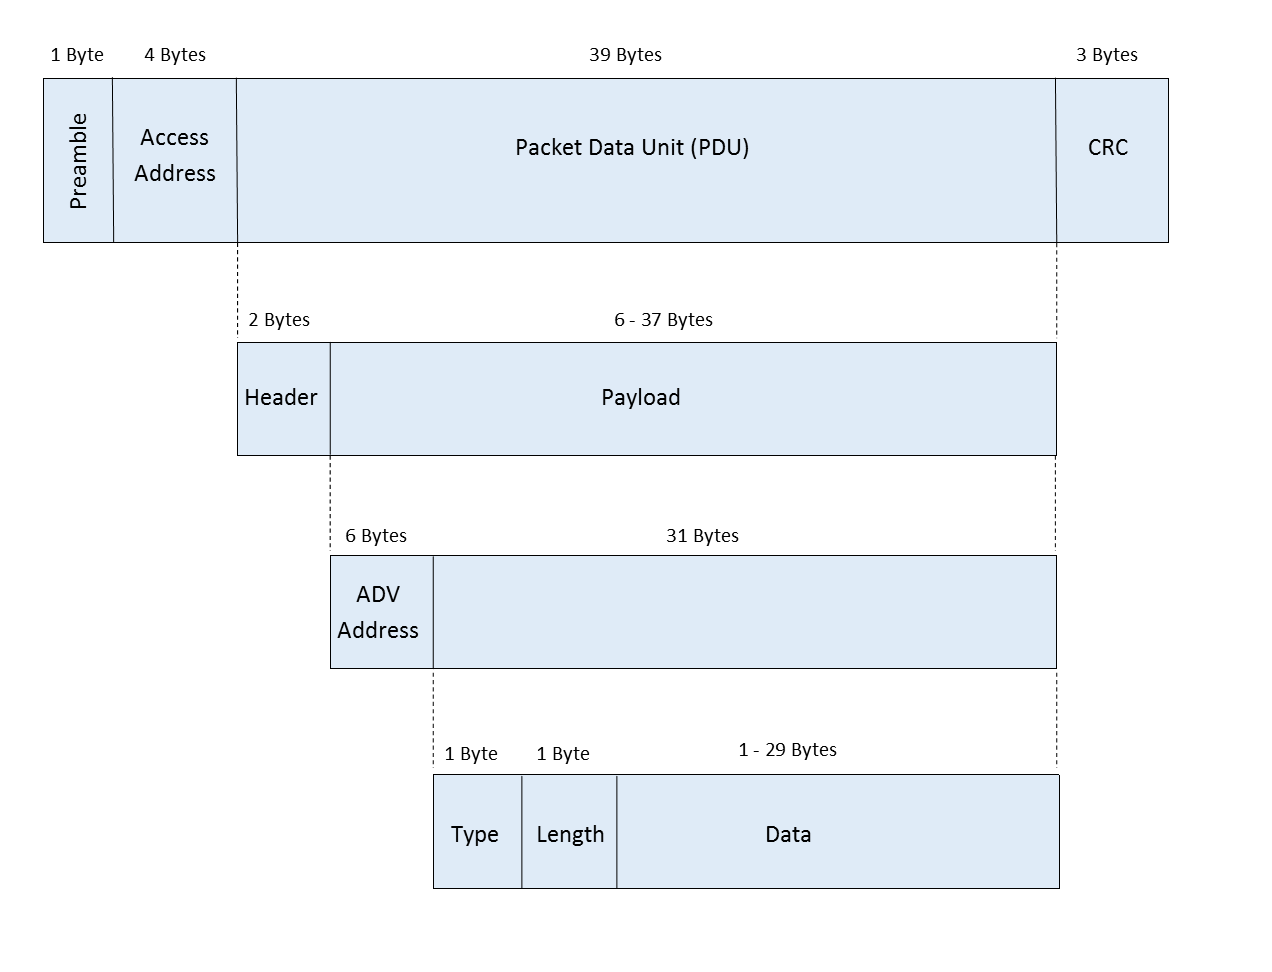
\includegraphics[width=\textwidth]{Images/chapter3/ble_pkt.png}
      \caption{BLE Advertisment Packet Structure}
      \label{fig:ble_pkt}
    \end{figure}
    \FloatBarrier

    \section{AODV BLE module}
    The attendance tracking applications are based on AODV's route discovery
    mechanism and so the main adaptations required for a Bluetooth Low Energy AODV module
    are discussed.

      \subsection{Advertisement Periods} \label{adv_periods}
    Unlike the multicast described in AODV's specification \cite{RFC3561},
    advertising in BLE is not instantaneous. As mentioned previously, a scanner's
    scan window must overlap with an advertiser's advertisement interval in order
    to receive data packets. Unlike connections, with broadcasting these intervals
    and windows are not synchronised. If a device wishes to broadcast a data packet,
    it is required to advertise that specific packet for a certain period. By selecting
    an appropriate period, the advertising device can be confident that the scanning
    windows of neighbouring devices will overlap with their advertisement interval
    within the specified period.

      \subsection{Packet Buffering}
    The receiving of an AODV control packet may require the receiver to broadcast
    a packet in response. As a result of the advertisement period discussed in section
    \ref{adv_periods}, packets which a device needs to send must be buffered.
    Without buffering, any currently advertising packets could go unreceived by
    not being broadcast for a sufficient amount of time.

    \section{Attendance Tracking}
    In the following sections the root node is the device tracking the attendance
    of user nodes and the root node's address is known globally.

      \subsection{Roll Call}
    The \textit{Roll Call} protocol is designed for lecture theatre-type scenarios.
    That is, a list of users is in our possession and we wish to determine which
    of these are present and which are not. An illustration of the protocol is
    provided in \ref{fig:roll_call}.

    \FloatBarrier
    \begin{figure}[ht]
      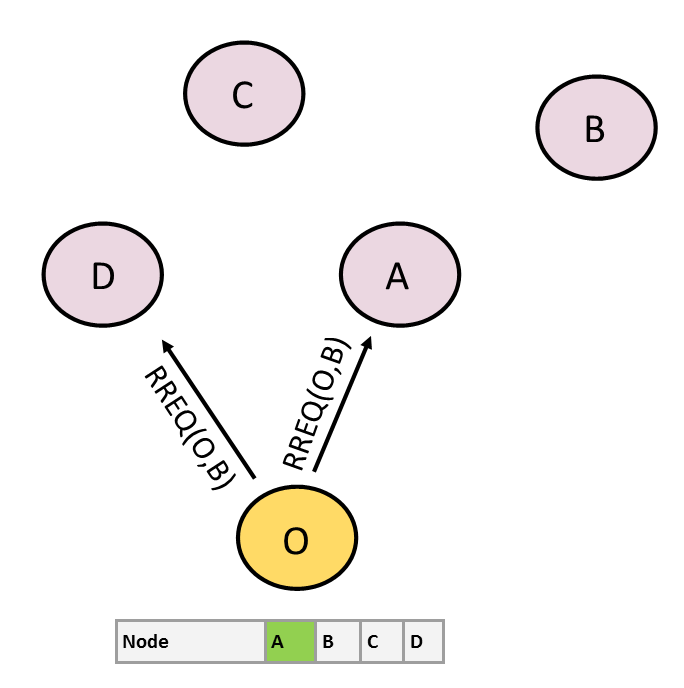
\includegraphics[scale=0.5]{Images/chapter3/roll_call.png}
      \caption{Roll Call}
      \label{fig:roll_call}
    \end{figure}
    \FloatBarrier

    To identify if a user is present, the root node broadcasts a RREQ into the
    network with the destination address set to that of the user. When a RREQ
    arrives in a node, if the node is not the destination, it re-broadcasts
    the RREQ according to AODV's specification. When a RREQ arrives at the
    destination node, they send a RREP back to the root node indicating their
    presence. If a RREP is not received before the end of the protocol, the user
    is counted as absent. The duration of the protocol is dependent on the size
    of the user list.

    In this protocol Low Power Listening radio duty cycling is performed.
    User nodes periodically scan to see if roll call is occurring. If they
    detect that it is occurring, they enter a high power state. The first
    RREQ sent by the root node has an advertisement period sufficiently long to
    ensure nearby nodes will detect it. This is similar to the method used by
    Box-MAC-2 in section \ref{box_mac}. The first RREQ is the preamble stream containing all
    the required data and is re-broadcast by receiving nodes.

      \subsection{Route to Zero}
    The \textit{Route-to-Zero} protocol is designed for scenarios in which the attendance
    of an otherwise unknown device can be taken. That is, a list of users is
    built during the protocol. An illustration of the protocol is provided in
    \ref{fig:route_to_zero}.

    \FloatBarrier
    \begin{figure}[ht]
      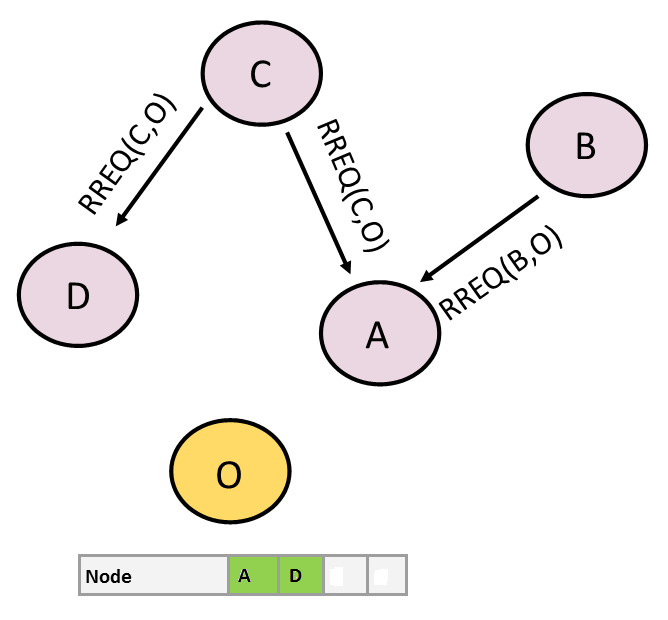
\includegraphics[scale=0.5]{Images/chapter3/route_to_zero.png}
      \caption{Route to Zero}
      \label{fig:route_to_zero}
    \end{figure}
    \FloatBarrier

    In this protocol, the responsibility of tracking attendance is placed on the
    users. User nodes attempt to discover a route to the root node by broadcasting
    a RREQ with the destination address set to that of the root node. When the
    RREQ arrives at the root, it adds the user to its list and sends a RREP
    back to the user node to acknowledge its presence.

    In this protocol, once again, Low Power Listening radio duty cycling is performed.
    User nodes periodically scan to see if Route-to-Zero is occurring. If they
    detect that it is occurring, they enter a high power state. The preamble in
    this scenario is a RREQ sent by the root with the destination and source address
    both equal to the root node's address. This RREQ is re-broadcast by all nodes
    that receive it. Upon receiving the RREQ, the user node enters a high power
    state and begins the protocol, identifying a route to the root node.

    \subsection{Design Discussion}
    There may exist the opportunity to use both the Roll Call and Route-to-Zero
    protocols in conjunction with one another. This might occur if the root node
    has a pre-determined list of users, additional users (not in the pre-determined list)
    can be in attendance, and users that might not all arrive at the same time.

    The route-to-zero protocol can be used initially, generating a list of present
    users. This list can be compared with the pre-determined list and
    if a user is missing, the Roll Call protocol can be initialised at a later point
    to verify the absence of the missing users.

    \section{Summary}
    When designing applications for BLE, careful consideration has to be taken
    with regards to the GAP communication types, whether broadcasting is sufficient
    or if connections are required. When broadcasting, the advertising intervals
    and scanning intervals and windows have to be selected with care. This is so
    the chance of a scan window overlapping with the advertisement interval is sufficiently
    high and so that too much power is not consumed. BLE advertisement packets have to
    be formed such that they adhere to the GAP packet specification, and it is
    important to choose advertisement data carefully as packets are limited in size.

    In order to translate AODV into a BLE module, some design decisions were required.
    The first of which is Advertisement Periods, to ensure that an advertisement
    packet is being broadcast for a sufficiently long time so that we can be
    confident that it will be received by neighbouring nodes. The second of which
    is Packet Buffering, a consequence of advertisement periods.

    Two protocols are proposed for attendance tracking, both of which are based
    on AODV's route discovery mechanism. The Roll Call protocol is designed for scenarios
    in which the attendance of a pre-determined group of users is being taken.
    The Route-to-zero protocol is designed for scenarios in which there is not
    a pre-determined group of users. These protocols can be used in conjunction
    if the scenario allows and requires it.
